% !TEX root = ../document.tex

\chapter{星基 ADS-B 原理概述}

\section{传统陆基 ADS-B 系统的不足}

世界上大多数地区都是不受控制的空域。在没有雷达覆盖的地区,称为 NRA(非雷达空域),如海洋空域、极地地区或结构上落后的大陆地区,地面站的安装要么不可能,要么太昂贵。现在,这些地区的监视手段是程序管制,即飞行员在到达某个固定的航路点时报告位置,或者应用 ADS-C (Automatic Dependent Surveillance – Contract,合同式自动相关监视),通过一个点对点的数据链连接(FANS1/A/Satcom),由于带宽有限,它仅每 15 分钟发送一次位置和其他航班信息。在这两种情况下都不可能实现无缝和连续的飞行监视,并且需要一个相对较大的飞行间隔来保证安全。

陆基 ADS-B 地面站越来越多地部署,但是覆盖区域通常限制在几百公里。以澳大利亚航空服务为例,建造了大量的 ADS-B 地面站最终覆盖了飞行高度 FL300 以上的区域。

由于技术、运行和政治条件的限制,对基于陆基 ADS-B 的空中交通活动的全球监视似乎有些力有未逮,主要体现在\upcite{h2}:

\begin{itemize}
    \item 海洋全部覆盖要求在大量的浮标上部署 ADS-B 地面站
    \item 地面全部覆盖要求在不可接近区域部署和运营 ADS-B 地面站
    \item 全球空域分散,各个空域由大量当地 ATC 提供商运作
    \item 在不稳定地区的政治障碍阻碍了任何跨国监管和运作
\end{itemize}

传统陆基 ADS-B 系统主要由空中机载发射机和地面接收基站组成,受制于系统布置限制,一般沿民航航路航线、机场终端区等陆地区域进行布置,很难实现对洋区、沙漠、高山峡谷等特殊地区的覆盖。据统计,全球 90\% 的区域没有实现飞行监视覆盖。基于星基的 ADS-B 系统可有效克服陆基 ADS-B 系统的不足,可用于陆基 ADS-B /雷达难以覆盖或无法覆盖的空域,从而形成一个全球无缝的 ADS-B 覆盖网络\upcite{z1}。

\section{星基 ADS-B 的实验背景}
\label{sec:space_based_ads-b_experiment_back}

2008 年,德国航空航天中心(DeutschesZentrumfürLuft-und Raumfahrt,DLR)开始调查接收低地球轨道(LEO,Low Earth Orbit)卫星上的飞机广播 1090ES ADS-B 信号。这促成了 DLR 的星基 ADS-B 项目(AOS,ADS-B over Satellite),目标是开发一个用于 IOD(在轨演示)的 ADS-B 载荷,从而证明基于卫星的 ADS-B 监视在全球范围内的可行性。

该 AOS 在轨演示器能够接收、解码和转发所有 S 模式下行链路格式报文,这包括 DF17 扩展震荡 ADS-B 报文和 DF11 全呼应答。AOS 的在轨演示器是在 ESA 的 PROBA-Vegetation 卫星任务框架内进行的,并于 2013 年 5 月 7 日在法属圭亚那 Kourou 由欧洲最新的 VEGA 运载火箭成功发射。

DLR 的这个在轨演示器是演示和验证天基空中交通监视的第一步。一颗卫星搭载了具有太空生存能力的 ADS-B 接收机,由于预算、时间、特殊资源和 PROBA-Vegetation 卫星在功率和几何形状方面的限制,该 ADS-B 载荷采用了相对简单的天线和接收机设计。在未来提供无缝全球覆盖的运营系统将包括这样一组卫星,每个卫星都配备有精密的多通道 ADS-B 接收机和天线\upcite{h2}。

AOS 项目是星基 ADS-B 的第一次实验并且已经证明了星基 ADS-B 的可行性。该 IOD 的实验结果将为未来星基空中交通监视的目标铺平道路。

\section{星基 ADS-B 的工作原理}

基于星基的 ADS-B 系统借助低轨道通信卫星的强大覆盖能力,将 ADS-B 收发信机安装到通信卫星上。通信卫星通过其 ADS-B 设备接收飞机发送的 ADS-B 报告,再通过卫星通信信道下传给卫星地面站,卫星地面站通过地面网络将 ADS-B 报告传递给地面相关实体(如 ATC 中心、航空公司等),实现 ADS-B 全球覆盖,完成对飞机的全球飞行追踪和实时监控\upcite{e1}。星基 ADS-B 系统的结构布局原理如图\ref{fig:satellite_ads-b_arichitecture}所示。

星基(Satellite-Based) ADS-B 系统,同样称为“天基(Space-Based)”、“卫星增强(Satellite-Augmented)”或者“卫星重传(Satellite-Retransmitted)” ADS-B 系统\upcite{h1}。

\begin{figure}[htbp]
\centering
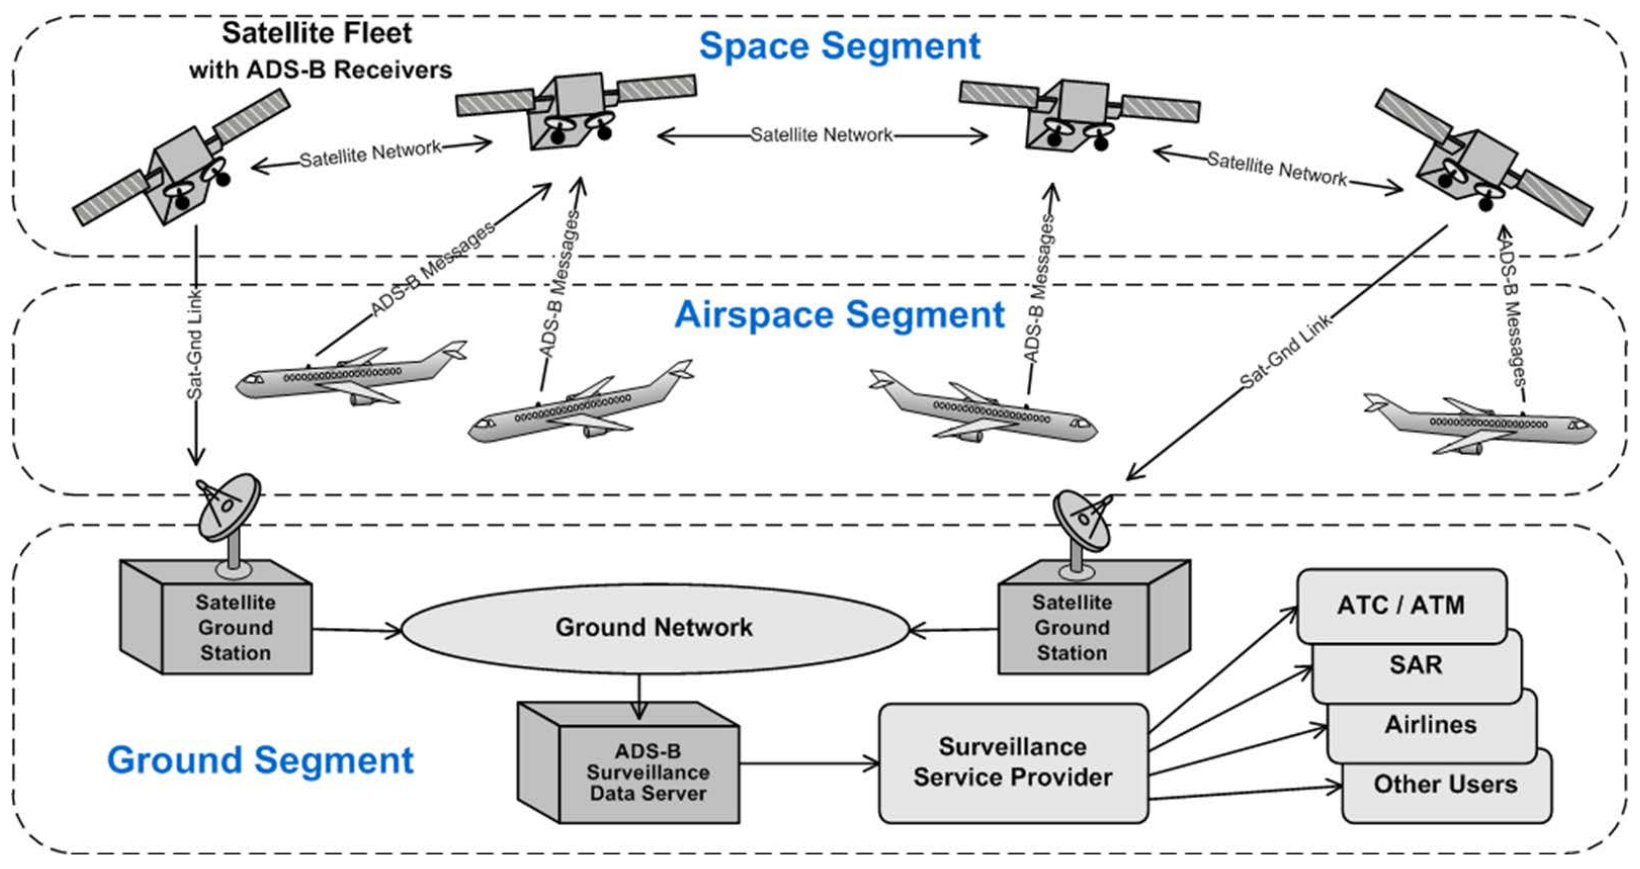
\includegraphics[width=15cm]{pic/satellite_ads-b_arichitecture.png}
\caption{星基 ADS-B 系统工作原理}
\label{fig:satellite_ads-b_arichitecture}
\end{figure}
